\documentclass{article}
\usepackage[utf8]{inputenc}
\usepackage{graphicx}

\title{Batch Analysis of Network Security Monitoring Data}
\author{Renu Tiwari, Jiang Xing Kun}
\date{January 2021}

\begin{document}

\maketitle

\section{Introduction}

This project is implementation for Batch Analysis of Network Security Monitoring Data. The goal is to load the data to a stream, transform to session data, save the session data to storage, do some lightweight analysis and visualize the results of the analysis.

\subsection{Data set}

The original data set shared was in network data format that is with .pcap extension. Wire-shark is used to load the data-set and then export the data to .csv file. The data set has 150k rows of data and 7 columns:
    \begin{enumerate}
    \item \textbf{No} - unique id for each row
    \item \textbf{Source} - The IP address of the source.
    \item \textbf{Destination} - The IP address of the destination/target.
    \item \textbf{Protocol} - The type of protocol used to communicate.
    \item \textbf{Length} - An integer value representing length of packets transferred.
    \item \textbf{Info} - Additional messages/information shared/communicated while transferring of the data.
    \end{enumerate}
   
\newpage
\section{System Architecture}
\subsection{System Architecture Diagram}

\begin{figure}[h!]
\centering
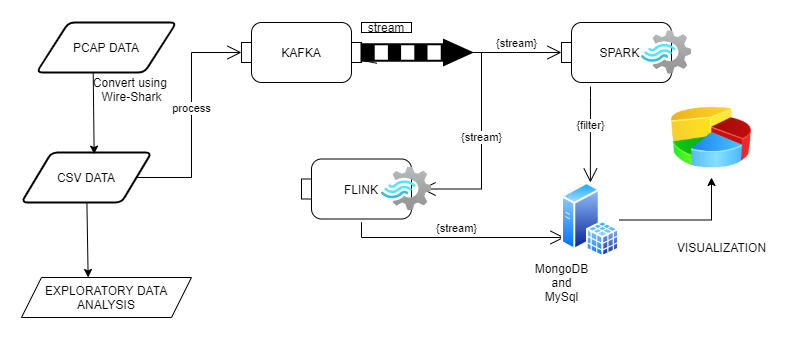
\includegraphics[scale=0.55]{Architecture.png}
\caption{System architecture diagram}
\label{fig:universe}
\end{figure}
 
\subsection{Data Conversion}
The initial data file was in .pcap format. Wire-shark is used to load the data and export it as .csv data. Wire-shark was used as to explore the use of software into this project and moreover it was a network monitoring related data. Thus, for initial first step of analysis wire-shark seemed to be a good choice.
\begin{figure}[h!]
\centering
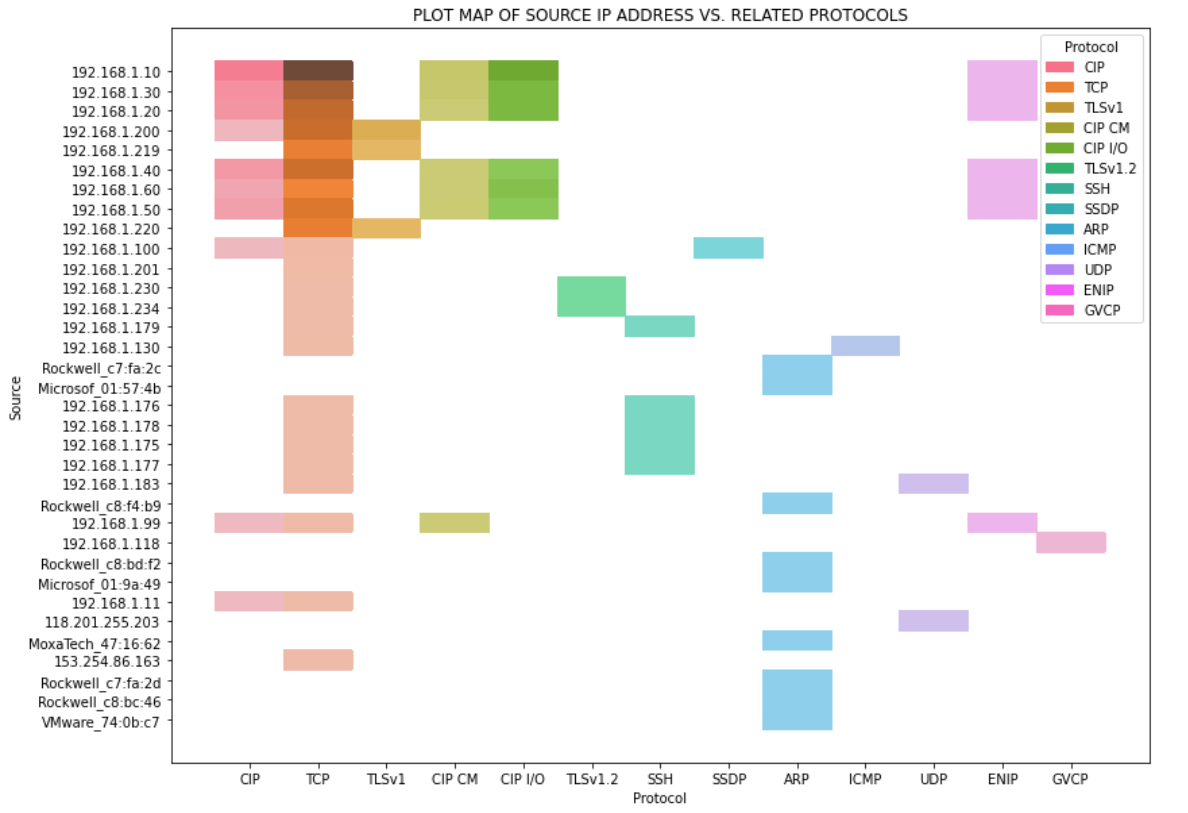
\includegraphics[scale=0.60]{source_protocol.PNG}
\caption{Source IP distribution over different protocols}
\label{fig:universe}
\end{figure}
\subsection{Pre-process Stage - Exploratory Data Analysis}
The .csv data then was loaded and processed using NetworkSecurity\_EDA.ipynb file. The data is loaded into a pandas data frame and then basic stastics are driven out. Few of the statistics are :
 \begin{enumerate}
    \item Count of different source IP address is 34.
    \item Count of different destination IP address is 42.
    \item Count of different protocols over which transmission happened is 13. The list of protocols is ['CIP' 'TCP' 'TLSv1' 'CIP CM' 'CIP I/O' 'TLSv1.2' 'SSH' 'SSDP' 'ARP'
 'ICMP' 'UDP' 'ENIP' 'GVCP']
    \item 
    Top 3 protocols via which data is communicated is -
    \begin{enumerate}
        \item Protocol  - Count
        \item TCP       - 95141
        \item CIP I/O   - 25320
        \item CIP       - 22188
    \end{enumerate}
    \item The most number of packets transferred are of length 64 and 60.
    \begin{enumerate}
        \item Packet Length - Count
        \item 64       - 25084
        \item 60   - 25084
        \item 86       - 9030
    \end{enumerate}

    \item The most communicated source and destination IP address is "192.168.1.10" with a total count of 33219.

    \item For experimentation, the Info part was also explored. Apparently, there also seems to be lot of useful info which can be used. Such as, below are some of the top information message communicated. Mostly, which are related to HMI\_PLANT, HMI\_PLANT\_AUTO or HMI\_PLANT\_RESET.

\begin{enumerate}
    \item Info Detail - Count 
    \item'HMI\_PLANT' - Service (0x4d) - 1184
\item Success: 'HMI\_PLANT' - Service -  1183
\item Success: 'HMI\_PLANT\_AUTO' - Service (0x4d) - 1137
\end{enumerate}
\end{enumerate}

\begin{figure}[h!]
\centering
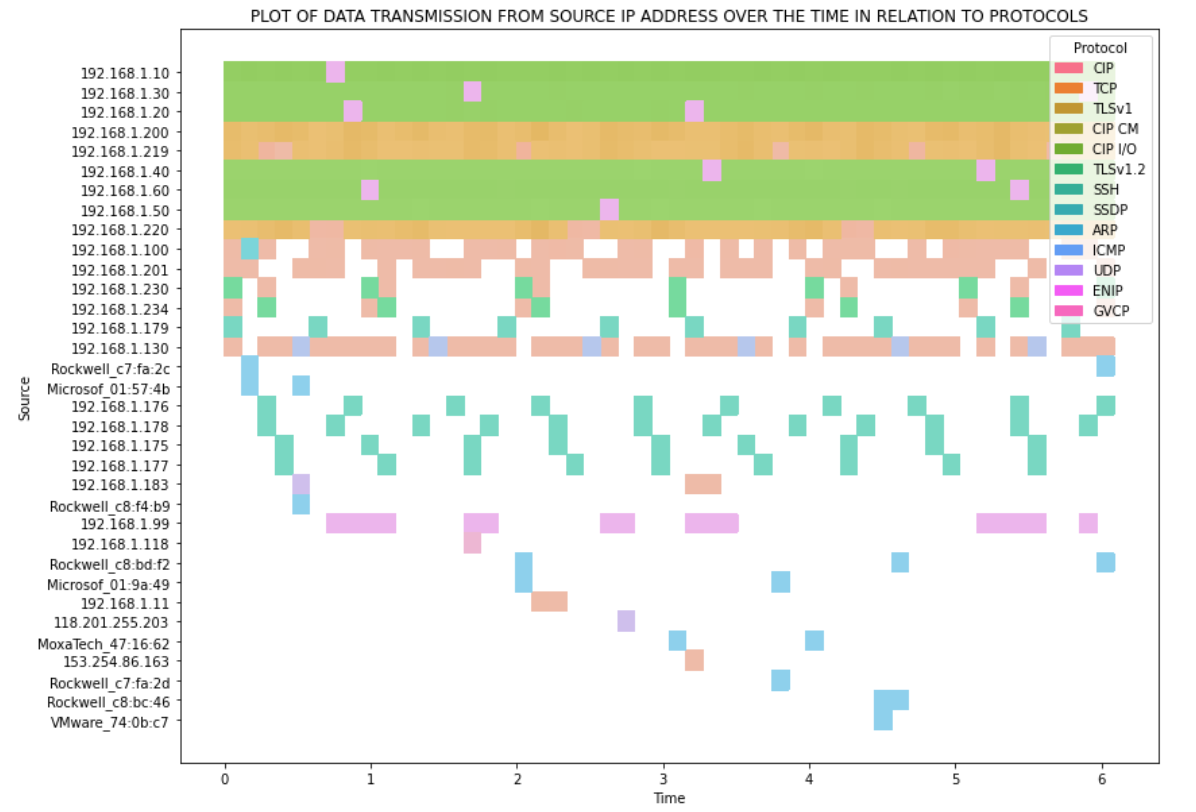
\includegraphics[scale=0.55]{source_time.PNG}
\caption{Source IP distribution over time}
\label{fig:universe}
\end{figure}

\subsection{Streaming}

\subsubsection{Kafka Streams}

As per Shree et al.(2017), it is "fast, scalable, distributed stream processing platform and fault tolerant messaging system." It is designed for low latency and high throughput.\cite{shree}. According to Bejeck (2018), "Kafka Streams is a library that allows you to perform per-event processing of records". Data is processed as it is available. Thus it is thought of a good option to use as a stream server.

The github repo contains folder named as "readData-sendKafka", reads the csv data and stream it using Kafka. The "Listener.java" file contains two topics named as "topic1" and "streaming". "KakfaPro" and "csv2KafkaStream" files uses these two listeners, Java's method BufferedReader to load csv to stream data. Once the kafka server starts, whole the dataset is visible at "localhost:8088/streamData" url.

\subsubsection{Java Spark Context Streams}
The data is received using Java Spark Context library. Kafka library has createDirectStream() methods which stream data into JavaInputDStream instance. Other methods such as flatmap and reduceByKey is used on the stream data.

\subsubsection{Flink}
For experimenting, Flink is also used to receive the stream data from Kafka. FlinkKafkaConsumer09 class loads the topic "topic1" and "streaming" into system. The major filtration is done on Spark.
\subsubsection{Filtering Data}
The filtrating of streamed data is done on two times and data is stored into respective tables. The RDD is read from JavaInputStream and for each RDD element, a check is used to see if the stream is using "TCP" protocol or not. If there's "TCP" protocol used, then data is processed further and stored in "tcp\_data" table.
The second type of filtration is done based on the length of streamed data. If the length of row is greater than 10 and it's communicated using protocol, then it's stored into "part5" table.

\begin{figure}[h!]
\centering
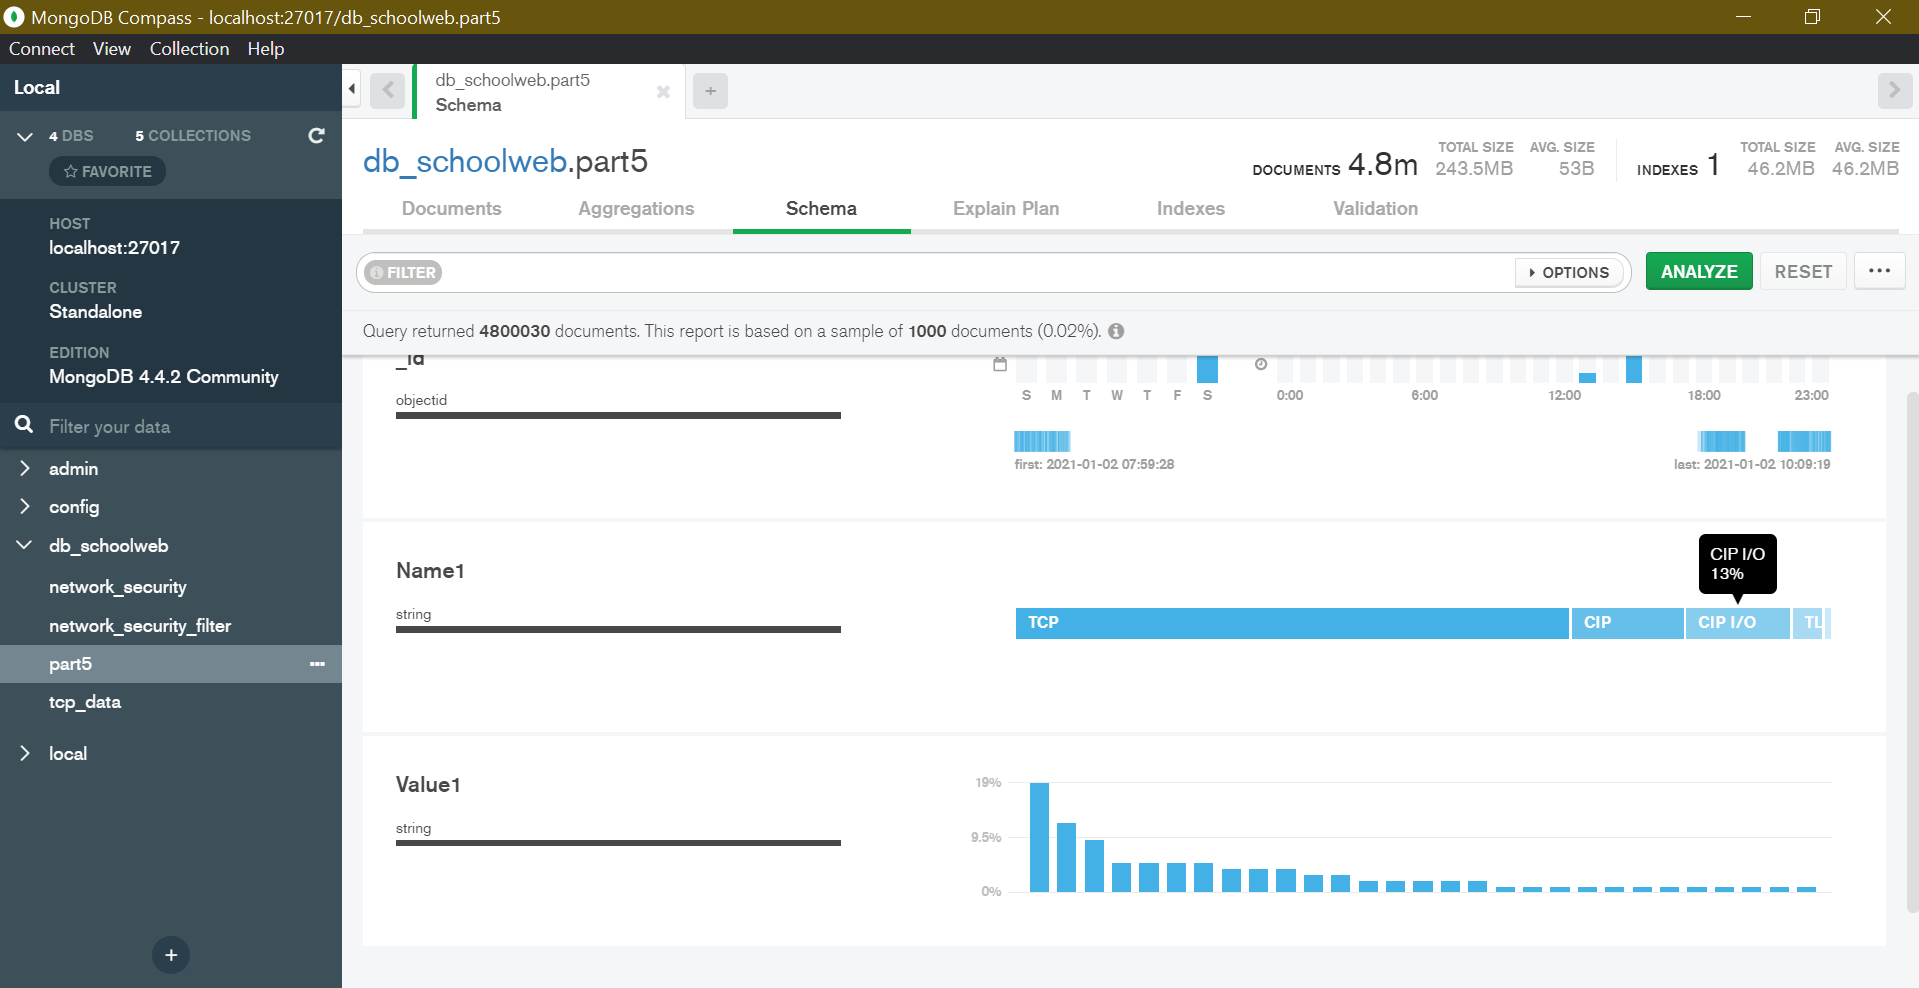
\includegraphics[scale=0.35]{part5_analysis_mongodb.png}
\caption{Analysis of data stored on basis of length}
\label{fig:universe}
\end{figure}

\subsection{MongoDB and MySQL}

For storage of data primarily, MongoDb is used. It is easily configurable and fast also. The spark module is written to stream the filtered data from above step to database. Initially, the data is stored into mysql database. Later and for final use, MongoDB is used. MongoDb Compass is used for hosting database. MongoClient is used with Java to load the collections and store the data into "tcp\_data". MySQL is used in storage of "part5" table.
\begin{figure}[h!]
\centering
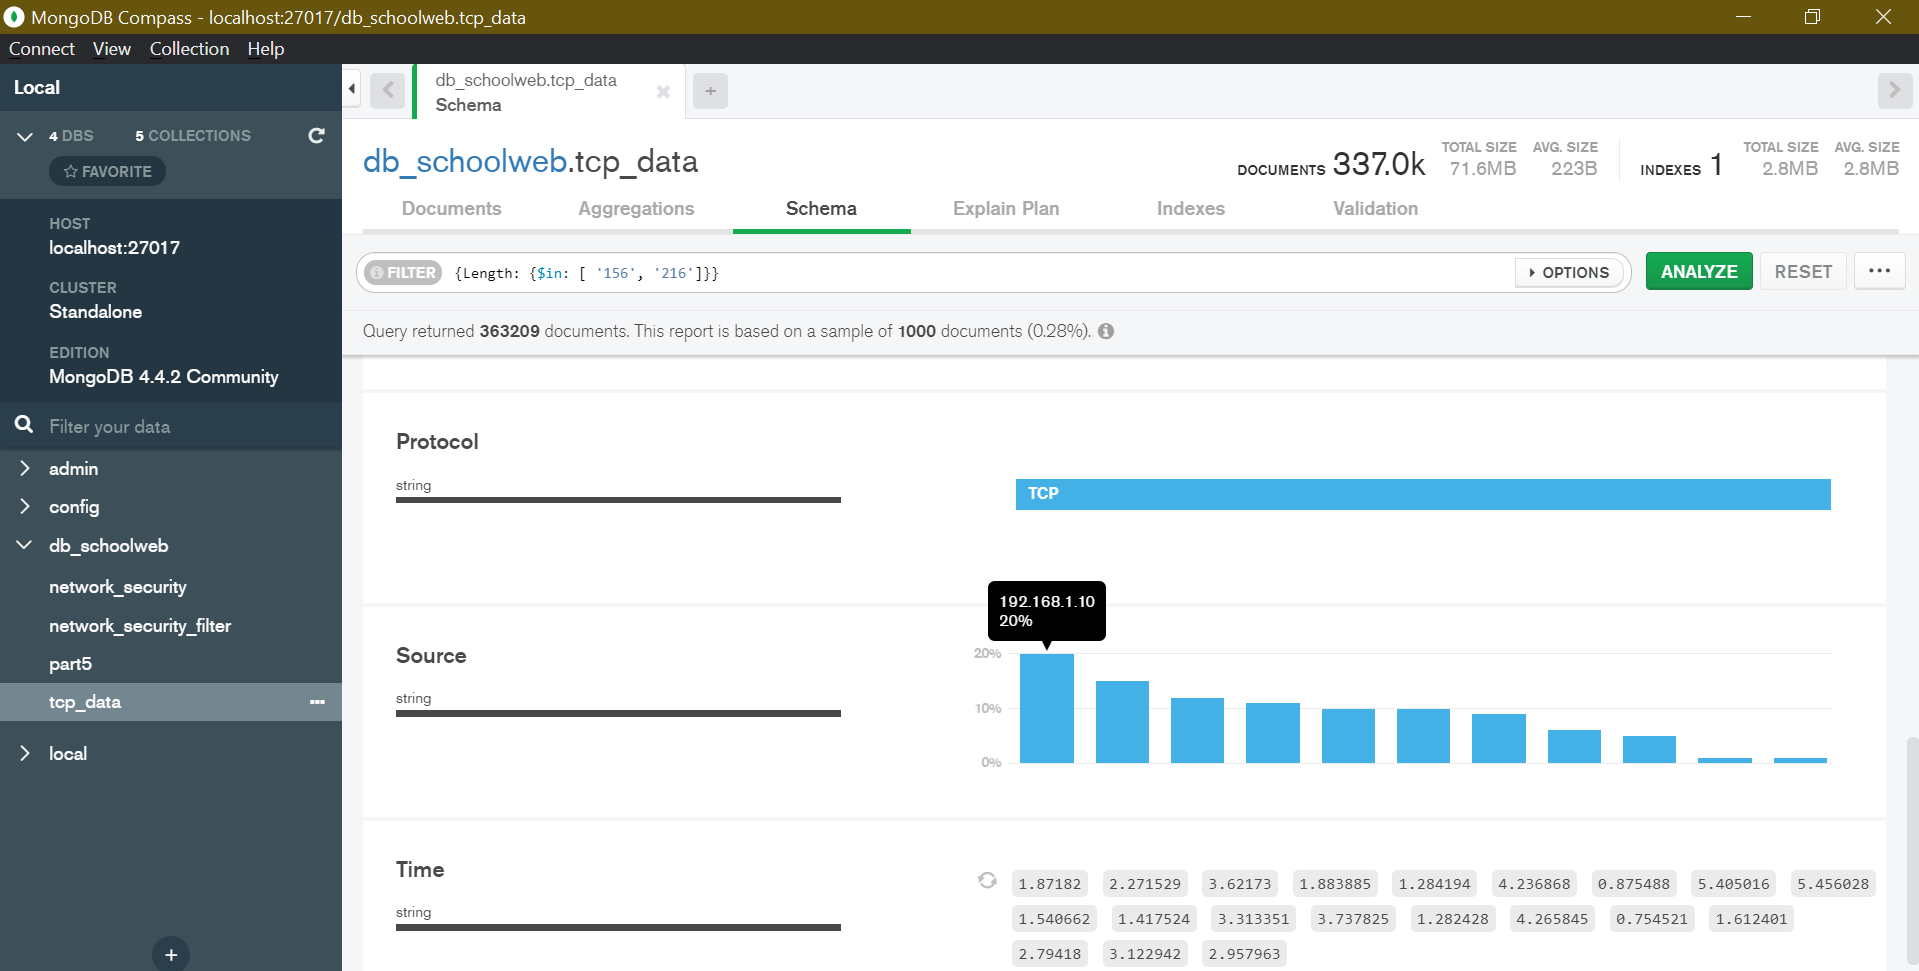
\includegraphics[scale=0.35]{tcp_analysis_mongoDb.png}
\caption{Analysis of TCP data on MongoDB}
\label{fig:universe}
\end{figure}


Kibana console was used to create, monitor and delete ElasticSearch indices, explore data loaded to ElasticSearch, and create dashboard to visualize the anomaly detection results.

\section{Execution Steps}
The overall pipeline of the project can be summarized in following steps:
\begin{itemize}
    \item Start the Zookeeper server (usually in port 2181)
    \item Start the Kafka server (usually in port 9092)
    \item Created two kafka topics named as "topic1" and "streaming" to load the csv data.
    \item Use csv2KafkaStream to load csv file to the kafka topic created earlier and see it on localhost:8088/streamData.
    \item Execute Spark-Kafka consumer connection application.
    \item Start MonDb server (usually on localhost: 27017)
    \item Create index using Kibana console to load the data to be visualized
    \item Open Dashboard.html to see the visualization.
\end{itemize}

\begin{figure}[h!]
\centering
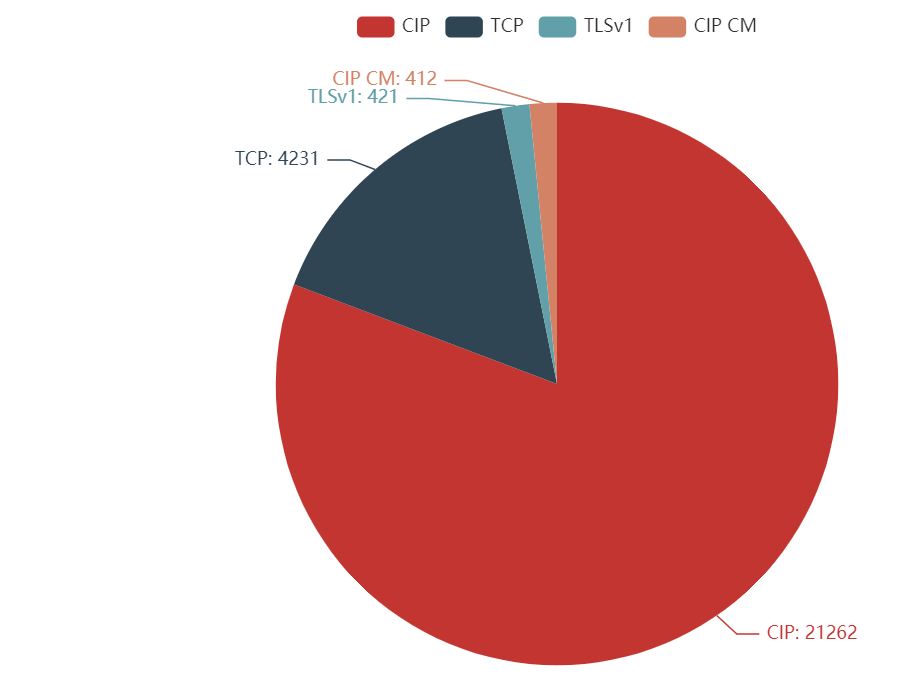
\includegraphics[scale=0.55]{Dashboard.PNG}
\caption{Pie chart visualization on basis of protocols}
\label{fig:universe}
\end{figure}

\section{Experiments}

\subsection{Converting JavaInputDStream to JavaRDD}

It was tried to use Spark inbuilt Filter methods on the streamed Kafka Data. As filter methods uses RDD to work on, it was tried to convert the stream to RDD. However, during the implementation of this idea, several problems were faced in typecasting and conversion of JavaInputDStream to JavaRDD as both takes different input. Also, Kafka streams data to Spark using directStream method. For using RDD, it would be beneficial if used Spark Streaming on both sides. However, RDDs are still executed from the stream data of input stream. It has method foreach(RDD), which was used to do user defined logical filtration.

\subsection{Analysis on Info Data}

The last part of the data contains the Info coloumn which contains various status codes and messages. As seen in EDA part, that there's high number of Info for HMI related codes.

\subsection{Considering Kafka as source and Spark as consumer}

A client-server architecture is tried to followed here. The Kafka side acts as server side to load the data into streams and then spark act as client to receive that stream and save it to database further. Also, this was done to experiment with  more technologies and how their communication works.

\subsection{Flink}

As a standalone task, a small experiment on using Flink was also done. The server side Kafka remains the same. But on consumer side, Flink is used to read the stream. Further, there's filteration and storage to Database is still in progress.

\subsection{Migrating from MySQL to MongoDB}

In previous section, it was shared about how collections and databases are used. Initially, MySQL was used to store the filer data. But then later, it was migrated to MongoDB as using MySQL was not in the scope of the project guidelines. Moreover installation, configuration and creating connection is relatively fast in MongoDB. Both these servers were hosted locally on personal computers.

%\section{References}

\begin{thebibliography}{9}

\bibitem{shree}
Shree, R., Choudhury, T., Gupta, S. and Kumar, P., (2017). KAFKA: The modern platform for data management and analysis in big data domain. 2017 2nd International Conference on Telecommunication and Networks (TEL-NET), 1. \url{https://ieeexplore.ieee.org/abstract/document/8343593/}

\bibitem{Bejeck}
Bejeck, B. (2018). Kafka Streams in Action: Real-time apps and microservices with the Kafka Streams API (1st ed.). Manning Publications.

\bibitem{rahasak}
Rahasak, Λ. (2020). Kafka and Zookeeper with Docker. https://medium.com/rahasak/kafka-and-zookeeper-with-docker-65cff2c2c34f

\end{thebibliography}

\end{document}